\chapter{Тағы да кесінділер дарағы туралы}

\index{кесінділер дарағы}

Кесінділер дарағы -- түрлі-түрлі есептерді шығару үшін қолданылатын 
икемді деректер құрылымы. Дегенмен кесінділер дарағына байланысты
кейбір тақырыптарды әлі өтпедік. Енді сол күрделі тақырыптарды өтетін уақыт
келді.

% A segment tree is a versatile data structure
% that can be used to solve a large number of algorithm problems.
% However, there are many topics related to segment trees
% that we have not touched yet.
% Now is time to discuss some more advanced variants
% of segment trees.

Осыған дейін біз кесінділер дарағының операцияларын 
дарақтың \emph{түбінен басына қарай} көтерілу арқылы жүзеге асырдық. 
Мысалы, аралық қосындысын төмендегідей есептедік (9.3-тарау):

% So far, we have implemented the operations
% of a segment tree by walking \emph{from bottom to top}
% in the tree.
% For example, we have calculated
% range sums as follows (Chapter 9.3):

\begin{lstlisting}
int sum(int a, int b) {
    a += n; b += n;
    int s = 0;
    while (a <= b) {
        if (a%2 == 1) s += tree[a++];
        if (b%2 == 0) s += tree[b--];
        a /= 2; b /= 2;
    }
    return s;
}
\end{lstlisting}

Бірақ күрделі кесінділер дарақтарында әдетте 
операцияларды керісінше, 
яғни \emph{жоғарыдан төменге} қарай орындау қажет. Осы тәсілді
қолдансақ, функция төмендегідей болады:

% However, in more advanced segment trees,
% it is often necessary to implement the operations
% in another way, \emph{from top to bottom}.
% Using this approach, the function becomes as follows:
\begin{lstlisting}
int sum(int a, int b, int k, int x, int y) {
    if (b < x || a > y) return 0;
    if (a <= x && y <= b) return tree[k];
    int d = (x+y)/2;
    return sum(a,b,2*k,x,d) + sum(a,b,2*k+1,d+1,y);
}
\end{lstlisting}

Енді кез келген $\texttt{sum}_q(a,b)$ мәнін 
($[a,b]$ аралығындағы жиым мәндерінің қосындысы)
келесідей есептейтін боламыз:
% Now we can calculate any value of $\texttt{sum}_q(a,b)$
% (the sum of array values in range $[a,b]$) as follows:
\begin{lstlisting}
int s = sum(a, b, 1, 0, n-1);
\end{lstlisting}

$k$ параметрі \texttt{дарақтағы} қазіргі позицияны көрсетеді. 
Басында $k$ 1-ге тең, себебі біз дарақтың түбірінен бастаймыз.
$[x,y]$ аралығы $k$ төбесіне сәйкес және басында $[0,n-1]$ аралығына тең.
Қосындыны есептеген кезде, егер $[x,y]$ аралығы $[a,b]$ аралығының сыртында 
болса, қосынды 0-ге тең. Ал егер $[x,y]$ аралығы толықтай $[a,b]$ аралығына 
кірсе, қосындыны \texttt{дарақтан} алсақ болады. Егер $[x,y]$ аралығының
кейбір бөлігі $[a,b]$ аралығына кірсе, ізденіс рекурсивті түрде 
$[x,y]$ аралығының оң мен сол жартысына жалғасады. Сол жартысы -- $[x,d]$
және оң жартысы -- $[d+1,y]$, мұндағы $d=\lfloor \frac{x+y}{2} \rfloor$. 

% The parameter $k$ indicates the current position
% in \texttt{tree}.
% Initially $k$ equals 1, because we begin
% at the root of the tree.
% The range $[x,y]$ corresponds to $k$
% and is initially $[0,n-1]$.
% When calculating the sum,
% if $[x,y]$ is outside $[a,b]$,
% the sum is 0,
% and if $[x,y]$ is completely inside $[a,b]$,
% the sum can be found in \texttt{tree}.
% If $[x,y]$ is partially inside $[a,b]$,
% the search continues recursively to the
% left and right half of $[x,y]$.
% The left half is $[x,d]$
% and the right half is $[d+1,y]$
% where $d=\lfloor \frac{x+y}{2} \rfloor$.

Келесі сурет  $\texttt{sum}_q(a,b)$ мәнін есептеу кезінде
ізденістің қалай жүретінін көрсетеді. Сұр төбелер рекурсия тоқтағанын 
көрсетеді және қосындыны дарақтың сол төбесінен алуымызға болады.

% The following picture shows how the search proceeds
% when calculating the value of $\texttt{sum}_q(a,b)$.
% The gray nodes indicate nodes where the recursion
% stops and the sum can be found in \texttt{tree}.

\begin{center}
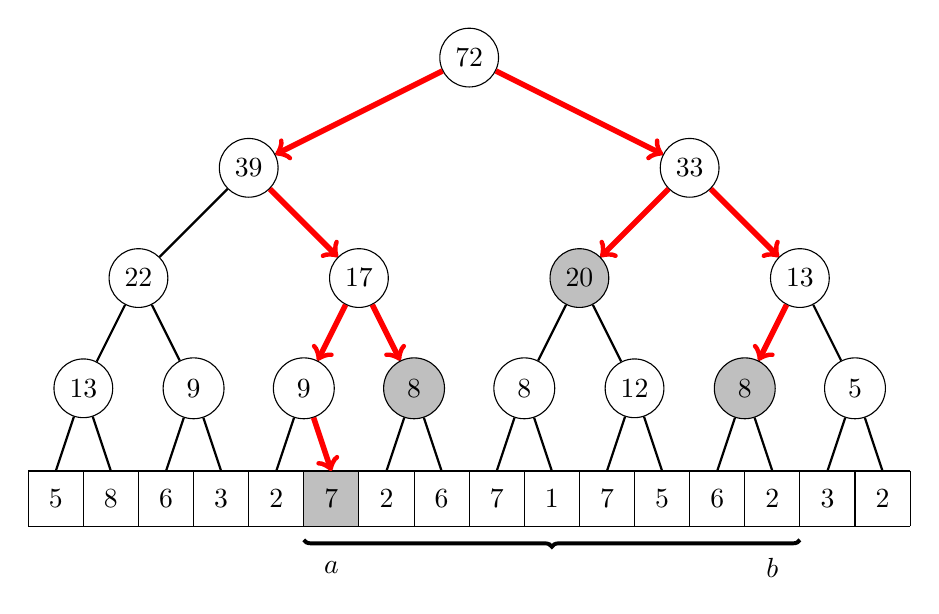
\begin{tikzpicture}[scale=0.7]
\fill[color=gray!50] (5,0) rectangle (6,1);
\draw (0,0) grid (16,1);

\node[anchor=center] at (0.5, 0.5) {5};
\node[anchor=center] at (1.5, 0.5) {8};
\node[anchor=center] at (2.5, 0.5) {6};
\node[anchor=center] at (3.5, 0.5) {3};
\node[anchor=center] at (4.5, 0.5) {2};
\node[anchor=center] at (5.5, 0.5) {7};
\node[anchor=center] at (6.5, 0.5) {2};
\node[anchor=center] at (7.5, 0.5) {6};
\node[anchor=center] at (8.5, 0.5) {7};
\node[anchor=center] at (9.5, 0.5) {1};
\node[anchor=center] at (10.5, 0.5) {7};
\node[anchor=center] at (11.5, 0.5) {5};
\node[anchor=center] at (12.5, 0.5) {6};
\node[anchor=center] at (13.5, 0.5) {2};
\node[anchor=center] at (14.5, 0.5) {3};
\node[anchor=center] at (15.5, 0.5) {2};

%\node[anchor=center] at (1,2.5) {13};

\node[draw, circle] (a) at (1,2.5) {13};
\path[draw,thick,-] (a) -- (0.5,1);
\path[draw,thick,-] (a) -- (1.5,1);
\node[draw, circle,minimum size=22pt] (b) at (3,2.5) {9};
\path[draw,thick,-] (b) -- (2.5,1);
\path[draw,thick,-] (b) -- (3.5,1);
\node[draw, circle,minimum size=22pt] (c) at (5,2.5) {9};
\path[draw,thick,-] (c) -- (4.5,1);
\path[draw,thick,-] (c) -- (5.5,1);
\node[draw, circle,fill=gray!50,minimum size=22pt] (d) at (7,2.5) {8};
\path[draw,thick,-] (d) -- (6.5,1);
\path[draw,thick,-] (d) -- (7.5,1);
\node[draw, circle,minimum size=22pt] (e) at (9,2.5) {8};
\path[draw,thick,-] (e) -- (8.5,1);
\path[draw,thick,-] (e) -- (9.5,1);
\node[draw, circle] (f) at (11,2.5) {12};
\path[draw,thick,-] (f) -- (10.5,1);
\path[draw,thick,-] (f) -- (11.5,1);
\node[draw, circle,fill=gray!50,minimum size=22pt] (g) at (13,2.5) {8};
\path[draw,thick,-] (g) -- (12.5,1);
\path[draw,thick,-] (g) -- (13.5,1);
\node[draw, circle,minimum size=22pt] (h) at (15,2.5) {5};
\path[draw,thick,-] (h) -- (14.5,1);
\path[draw,thick,-] (h) -- (15.5,1);

\node[draw, circle] (i) at (2,4.5) {22};
\path[draw,thick,-] (i) -- (a);
\path[draw,thick,-] (i) -- (b);
\node[draw, circle] (j) at (6,4.5) {17};
\path[draw,thick,-] (j) -- (c);
\path[draw,thick,-] (j) -- (d);
\node[draw, circle,fill=gray!50] (k) at (10,4.5) {20};
\path[draw,thick,-] (k) -- (e);
\path[draw,thick,-] (k) -- (f);
\node[draw, circle] (l) at (14,4.5) {13};
\path[draw,thick,-] (l) -- (g);
\path[draw,thick,-] (l) -- (h);

\node[draw, circle] (m) at (4,6.5) {39};
\path[draw,thick,-] (m) -- (i);
\path[draw,thick,-] (m) -- (j);
\node[draw, circle] (n) at (12,6.5) {33};
\path[draw,thick,-] (n) -- (k);
\path[draw,thick,-] (n) -- (l);

\node[draw, circle] (o) at (8,8.5) {72};
\path[draw,thick,-] (o) -- (m);
\path[draw,thick,-] (o) -- (n);

\path[draw=red,thick,->,line width=2pt] (o) -- (m);
\path[draw=red,thick,->,line width=2pt] (o) -- (n);

\path[draw=red,thick,->,line width=2pt] (m) -- (j);
\path[draw=red,thick,->,line width=2pt] (j) -- (c);
\path[draw=red,thick,->,line width=2pt] (j) -- (d);
\path[draw=red,thick,->,line width=2pt] (c) -- (5.5,1);

\path[draw=red,thick,->,line width=2pt] (n) -- (k);
\path[draw=red,thick,->,line width=2pt] (n) -- (l);

\path[draw=red,thick,->,line width=2pt] (l) -- (g);

\draw [decoration={brace}, decorate, line width=0.5mm] (14,-0.25) -- (5,-0.25);

\node at (5.5,-0.75) {$a$};
\node at (13.5,-0.75) {$b$};
\end{tikzpicture}
\end{center}

Бұл код та операцияларды өңдеу үшін
$O(\log n)$ уақыт алады, өйткені барлық өтіп шығатын 
төбелердің саны -- $O(\log n)$.
% Also in this implementation,
% operations take $O(\log n)$ time,
% because the total number of visited nodes is $O(\log n)$.

\section{Жалқау таратылу}

\index{жалқау таратылу}
\index{жалқау кесінділер дарағы}

\key{Жалқау таратылу} арқылы аралық жаңартулар \emph{мен}
аралық сұратымдарды $O(\log n)$ уақытта қолдайтын кесінділер
дарағын құрастыруға болады. Идеясы жаңарту және сұратым 
операцияларын жоғарыдан төменге қарай өңдеуге және жаңартуларды
керек кезінде ғана \emph{жалқау} түрде төменге таратуға негізделеді.


% Using \key{lazy propagation}, we can build
% a segment tree that supports \emph{both} range updates
% and range queries in $O(\log n)$ time.
% The idea is to perform updates and queries
% from top to bottom and perform updates
% \emph{lazily} so that they are propagated
% down the tree only when it is necessary.

Жалқау кесінділер дарағындағы төбе екі түрлі ақпаратты
сақтайды. Біріншіден, қарапайым кесінділер дарағы сияқты
әр төбе сәйкес ішжиымның 
қосындысын немесе ішжиымға қатысты басқа мәнді сақтайды.
Екіншіден, төбе ұлдарына таратылмаған жалқау жаңартуларға қатысты 
ақпаратты сақтауы мүмкін.

% In a lazy segment tree, nodes contain two types of
% information.
% Like in an ordinary segment tree,
% each node contains the sum or some other value
% related to the corresponding subarray.
% In addition, the node may contain information
% related to lazy updates, which has not been
% propagated to its children.

Аралық сұратымдардың екі түрі бар. 
Аралықтағы барлық жиым мәндері бір мәнге \emph{арттырылады} 
немесе жиым мәндеріне бір мән \emph{меншіктеледі}.
Екі операцияны да ұқсас идея арқылы жүзеге асыруға болады,
тіпті екі операцияны бір уақытта қолдайтын дарақты да
құруға болады. 


% There are two types of range updates:
% each array value in the range is either
% \emph{increased} by some value
% or \emph{assigned} some value.
% Both operations can be implemented using
% similar ideas, and it is even possible to construct
% a tree that supports both operations at the same time.

\subsubsection{Жалқау кесінділер дарағы}

$[a,b]$ аралығын тұрақты санға арттыратын және
$[a,b]$ аралығындағы мәндерінің қосындысын табатын кесінділер дарағын
мысал ретінде қарастырайық. 

% Let us consider an example where our goal is to
% construct a segment tree that supports
% two operations: increasing each value in
% $[a,b]$ by a constant and calculating the sum of
% values in $[a,b]$.

Біз әр төбеде екі мән $s/z$ болатындай дарақты
құрастырамыз. Мұндағы $s$ аралықтағы мәндердің 
қосындысын белгілесе, $z$ жалқау жаңарту мәнін 
белгілейді, яғни сол аралықтағы мәндердің барлығы
$z$-ке арттырылуы тиіс. Келесі дарақта барлық
төбелерде $z=0$, яғни әзірге жалқау жаңартулар жоқ.

% We will construct a tree where each node
% has two values $s/z$:
% $s$ denotes the sum of values in the range,
% and $z$ denotes the value of a lazy update,
% which means that all values in the range
% should be increased by $z$.
% In the following tree, $z=0$ in all nodes,
% so there are no ongoing lazy updates.
\begin{center}
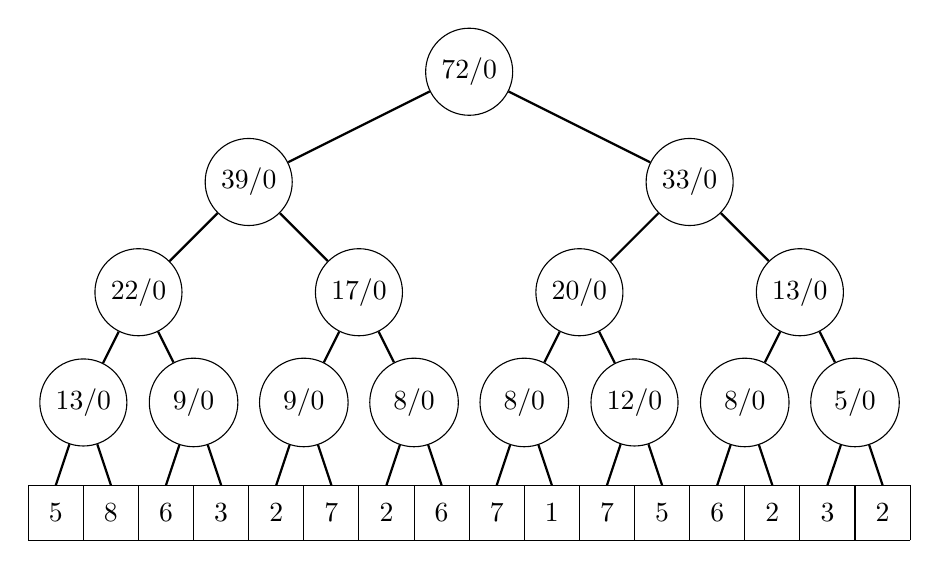
\begin{tikzpicture}[scale=0.7]
\draw (0,0) grid (16,1);

\node[anchor=center] at (0.5, 0.5) {5};
\node[anchor=center] at (1.5, 0.5) {8};
\node[anchor=center] at (2.5, 0.5) {6};
\node[anchor=center] at (3.5, 0.5) {3};
\node[anchor=center] at (4.5, 0.5) {2};
\node[anchor=center] at (5.5, 0.5) {7};
\node[anchor=center] at (6.5, 0.5) {2};
\node[anchor=center] at (7.5, 0.5) {6};
\node[anchor=center] at (8.5, 0.5) {7};
\node[anchor=center] at (9.5, 0.5) {1};
\node[anchor=center] at (10.5, 0.5) {7};
\node[anchor=center] at (11.5, 0.5) {5};
\node[anchor=center] at (12.5, 0.5) {6};
\node[anchor=center] at (13.5, 0.5) {2};
\node[anchor=center] at (14.5, 0.5) {3};
\node[anchor=center] at (15.5, 0.5) {2};

\node[draw, circle] (a) at (1,2.5) {13/0};
\path[draw,thick,-] (a) -- (0.5,1);
\path[draw,thick,-] (a) -- (1.5,1);
\node[draw, circle,minimum size=32pt] (b) at (3,2.5) {9/0};
\path[draw,thick,-] (b) -- (2.5,1);
\path[draw,thick,-] (b) -- (3.5,1);
\node[draw, circle,minimum size=32pt] (c) at (5,2.5) {9/0};
\path[draw,thick,-] (c) -- (4.5,1);
\path[draw,thick,-] (c) -- (5.5,1);
\node[draw, circle,minimum size=32pt] (d) at (7,2.5) {8/0};
\path[draw,thick,-] (d) -- (6.5,1);
\path[draw,thick,-] (d) -- (7.5,1);
\node[draw, circle,minimum size=32pt] (e) at (9,2.5) {8/0};
\path[draw,thick,-] (e) -- (8.5,1);
\path[draw,thick,-] (e) -- (9.5,1);
\node[draw, circle] (f) at (11,2.5) {12/0};
\path[draw,thick,-] (f) -- (10.5,1);
\path[draw,thick,-] (f) -- (11.5,1);
\node[draw, circle,minimum size=32pt] (g) at (13,2.5) {8/0};
\path[draw,thick,-] (g) -- (12.5,1);
\path[draw,thick,-] (g) -- (13.5,1);
\node[draw, circle,minimum size=32pt] (h) at (15,2.5) {5/0};
\path[draw,thick,-] (h) -- (14.5,1);
\path[draw,thick,-] (h) -- (15.5,1);

\node[draw, circle] (i) at (2,4.5) {22/0};
\path[draw,thick,-] (i) -- (a);
\path[draw,thick,-] (i) -- (b);
\node[draw, circle] (j) at (6,4.5) {17/0};
\path[draw,thick,-] (j) -- (c);
\path[draw,thick,-] (j) -- (d);
\node[draw, circle] (k) at (10,4.5) {20/0};
\path[draw,thick,-] (k) -- (e);
\path[draw,thick,-] (k) -- (f);
\node[draw, circle] (l) at (14,4.5) {13/0};
\path[draw,thick,-] (l) -- (g);
\path[draw,thick,-] (l) -- (h);

\node[draw, circle] (m) at (4,6.5) {39/0};
\path[draw,thick,-] (m) -- (i);
\path[draw,thick,-] (m) -- (j);
\node[draw, circle] (n) at (12,6.5) {33/0};
\path[draw,thick,-] (n) -- (k);
\path[draw,thick,-] (n) -- (l);

\node[draw, circle] (o) at (8,8.5) {72/0};
\path[draw,thick,-] (o) -- (m);
\path[draw,thick,-] (o) -- (n);
\end{tikzpicture}
\end{center}

$[a,b]$ аралығындағы элементтер $u$-ге арттырылған кезде
біз түбірден жапырақтарға қарай жүріп, дарақтағы төбелерді
келесі ретпен өзгерте аламыз.
Егер төбенің $[x,y]$ аралығы толықтай $[a,b]$ аралығына кірсе,
төбенің $z$ мәнін $u$-ге арттырамыз және тоқтаймыз. 
Ал егер $[x,y]$ аралығының
кейбір бөлігі $[a,b]$ аралығына кірсе, онда төбенің
$s$ мәнін $hu$ мәніне арттырамыз, мұндағы $h$ -- $[a,b]$ мен 
$[x,y]$ аралықтарының қиылысу өлшемі, және дарақ
бойынша өтуімізді рекурсивті түрде жалғастырамыз. 


% When the elements in $[a,b]$ are increased by $u$,
% we walk from the root towards the leaves
% and modify the nodes of the tree as follows:
% If the range $[x,y]$ of a node is
% completely inside $[a,b]$,
% we increase the $z$ value of the node by $u$ and stop.
% If $[x,y]$ only partially belongs to $[a,b]$,
% we increase the $s$ value of the node by $hu$,
% where $h$ is the size of the intersection of $[a,b]$
% and $[x,y]$, and continue our walk recursively in the tree.

Мысалы, келесі суретте $[a,b]$ аралықтағы элементтерді 2-ге 
арттырғаннан кейінгі дарақ бейнеленген:

% For example, the following picture shows the tree after
% increasing the elements in $[a,b]$ by 2:
\begin{center}
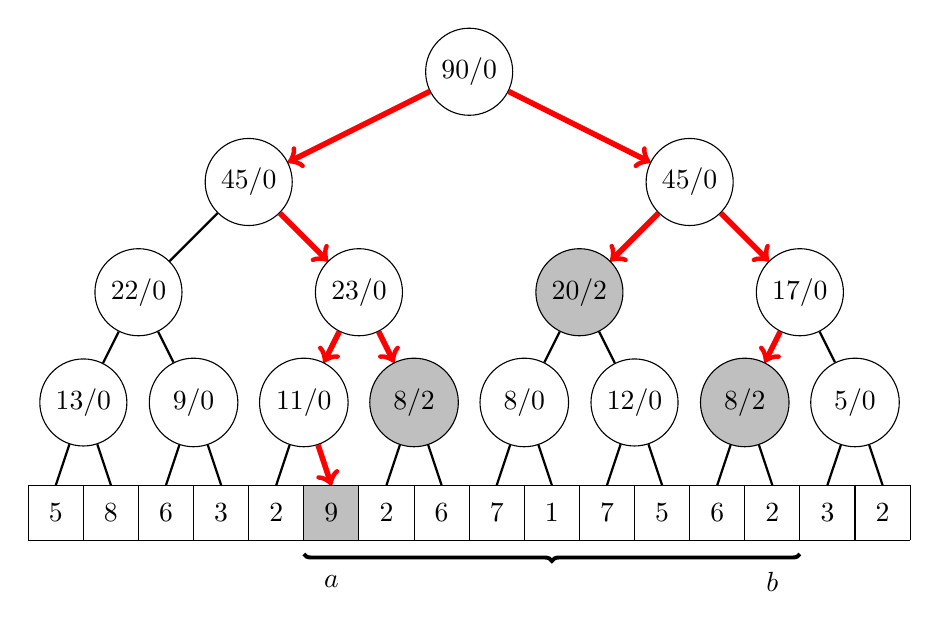
\begin{tikzpicture}[scale=0.7]
\fill[color=gray!50] (5,0) rectangle (6,1);
\draw (0,0) grid (16,1);

\node[anchor=center] at (0.5, 0.5) {5};
\node[anchor=center] at (1.5, 0.5) {8};
\node[anchor=center] at (2.5, 0.5) {6};
\node[anchor=center] at (3.5, 0.5) {3};
\node[anchor=center] at (4.5, 0.5) {2};
\node[anchor=center] at (5.5, 0.5) {9};
\node[anchor=center] at (6.5, 0.5) {2};
\node[anchor=center] at (7.5, 0.5) {6};
\node[anchor=center] at (8.5, 0.5) {7};
\node[anchor=center] at (9.5, 0.5) {1};
\node[anchor=center] at (10.5, 0.5) {7};
\node[anchor=center] at (11.5, 0.5) {5};
\node[anchor=center] at (12.5, 0.5) {6};
\node[anchor=center] at (13.5, 0.5) {2};
\node[anchor=center] at (14.5, 0.5) {3};
\node[anchor=center] at (15.5, 0.5) {2};

\node[draw, circle] (a) at (1,2.5) {13/0};
\path[draw,thick,-] (a) -- (0.5,1);
\path[draw,thick,-] (a) -- (1.5,1);
\node[draw, circle,minimum size=32pt] (b) at (3,2.5) {9/0};
\path[draw,thick,-] (b) -- (2.5,1);
\path[draw,thick,-] (b) -- (3.5,1);
\node[draw, circle,minimum size=32pt] (c) at (5,2.5) {11/0};
\path[draw,thick,-] (c) -- (4.5,1);
\path[draw,thick,-] (c) -- (5.5,1);
\node[draw, circle,fill=gray!50,minimum size=32pt] (d) at (7,2.5) {8/2};
\path[draw,thick,-] (d) -- (6.5,1);
\path[draw,thick,-] (d) -- (7.5,1);
\node[draw, circle,minimum size=32pt] (e) at (9,2.5) {8/0};
\path[draw,thick,-] (e) -- (8.5,1);
\path[draw,thick,-] (e) -- (9.5,1);
\node[draw, circle] (f) at (11,2.5) {12/0};
\path[draw,thick,-] (f) -- (10.5,1);
\path[draw,thick,-] (f) -- (11.5,1);
\node[draw, circle,fill=gray!50,minimum size=32pt] (g) at (13,2.5) {8/2};
\path[draw,thick,-] (g) -- (12.5,1);
\path[draw,thick,-] (g) -- (13.5,1);
\node[draw, circle,minimum size=32pt] (h) at (15,2.5) {5/0};
\path[draw,thick,-] (h) -- (14.5,1);
\path[draw,thick,-] (h) -- (15.5,1);

\node[draw, circle] (i) at (2,4.5) {22/0};
\path[draw,thick,-] (i) -- (a);
\path[draw,thick,-] (i) -- (b);
\node[draw, circle] (j) at (6,4.5) {23/0};
\path[draw,thick,-] (j) -- (c);
\path[draw,thick,-] (j) -- (d);
\node[draw, circle,fill=gray!50] (k) at (10,4.5) {20/2};
\path[draw,thick,-] (k) -- (e);
\path[draw,thick,-] (k) -- (f);
\node[draw, circle] (l) at (14,4.5) {17/0};
\path[draw,thick,-] (l) -- (g);
\path[draw,thick,-] (l) -- (h);

\node[draw, circle] (m) at (4,6.5) {45/0};
\path[draw,thick,-] (m) -- (i);
\path[draw,thick,-] (m) -- (j);
\node[draw, circle] (n) at (12,6.5) {45/0};
\path[draw,thick,-] (n) -- (k);
\path[draw,thick,-] (n) -- (l);

\node[draw, circle] (o) at (8,8.5) {90/0};
\path[draw,thick,-] (o) -- (m);
\path[draw,thick,-] (o) -- (n);

\path[draw=red,thick,->,line width=2pt] (o) -- (m);
\path[draw=red,thick,->,line width=2pt] (o) -- (n);

\path[draw=red,thick,->,line width=2pt] (m) -- (j);
\path[draw=red,thick,->,line width=2pt] (j) -- (c);
\path[draw=red,thick,->,line width=2pt] (j) -- (d);
\path[draw=red,thick,->,line width=2pt] (c) -- (5.5,1);

\path[draw=red,thick,->,line width=2pt] (n) -- (k);
\path[draw=red,thick,->,line width=2pt] (n) -- (l);

\path[draw=red,thick,->,line width=2pt] (l) -- (g);

\draw [decoration={brace}, decorate, line width=0.5mm] (14,-0.25) -- (5,-0.25);

\node at (5.5,-0.75) {$a$};
\node at (13.5,-0.75) {$b$};
\end{tikzpicture}
\end{center}

Сондай-ақ біз $[a,b]$ аралығындағы элементтердің қосындысын 
дарақты жоғарыдан төменге қарай өту арқылы есептейміз. Егер төбенің 
$[x,y]$ аралығы толықтай $[a,b]$ аралығына кірсе, біз қосындыға 
төбенің $s$ мәнін қосамыз. Әйтпесе ізденісті рекурсивті түрде 
дарақтың төменіне қарай жалғастырамыз. 


% We also calculate the sum of elements in a range $[a,b]$
% by walking in the tree from top to bottom.
% If the range $[x,y]$ of a node completely belongs
% to $[a,b]$, we add the $s$ value of the node to the sum.
% Otherwise, we continue the search recursively
% downwards in the tree.

Жаңартуда да, сұратымда да 
әрдайым төбені өңдеуден бұрын жалқау жаңартудың 
мәні төбенің ұлдарына таратылады. Демек 
жаңартулар керек болған жағдайда ғана төменге
қарай таратылады, ал бұл операциялардың оңтайлы
болуына кепілдік береді. 


% Both in updates and queries,
% the value of a lazy update is always propagated
% to the children of the node
% before processing the node.
% The idea is that updates will be propagated
% downwards only when it is necessary,
% which guarantees that the operations are always efficient.

Келесі сурет $\texttt{sum}_a(a,b)$ мәнін есептеген кезде
дарақ қалай өзгеретінін көрсетеді. Төртбұрыш жалқау жаңартулардың
төменге таратылуына байланысты өзгерген төбелерді көрсетеді. 

% The following picture shows how the tree changes
% when we calculate the value of $\texttt{sum}_a(a,b)$.
% The rectangle shows the nodes whose values change,
% because a lazy update is propagated downwards.

\begin{center}
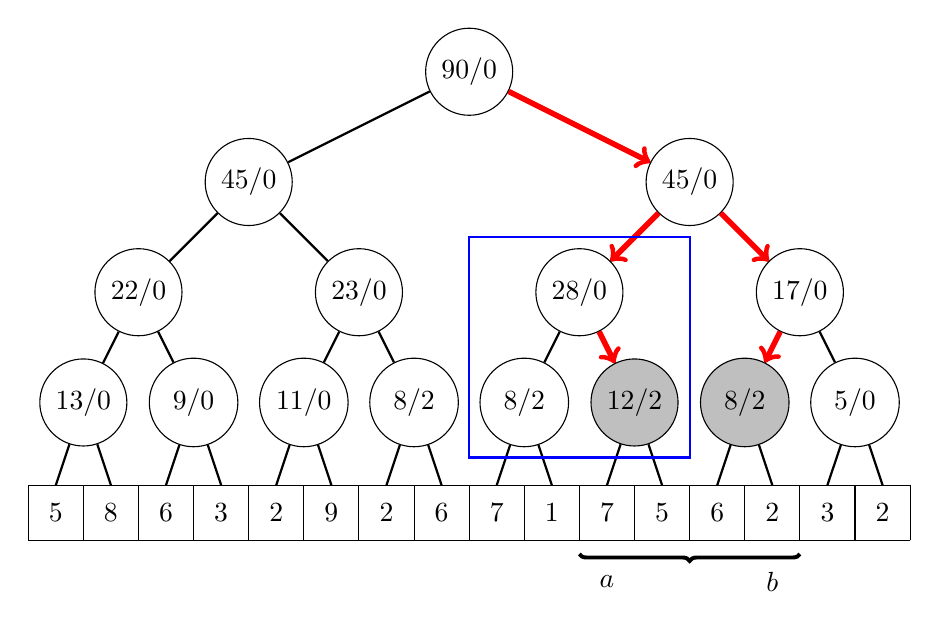
\begin{tikzpicture}[scale=0.7]
\draw (0,0) grid (16,1);

\node[anchor=center] at (0.5, 0.5) {5};
\node[anchor=center] at (1.5, 0.5) {8};
\node[anchor=center] at (2.5, 0.5) {6};
\node[anchor=center] at (3.5, 0.5) {3};
\node[anchor=center] at (4.5, 0.5) {2};
\node[anchor=center] at (5.5, 0.5) {9};
\node[anchor=center] at (6.5, 0.5) {2};
\node[anchor=center] at (7.5, 0.5) {6};
\node[anchor=center] at (8.5, 0.5) {7};
\node[anchor=center] at (9.5, 0.5) {1};
\node[anchor=center] at (10.5, 0.5) {7};
\node[anchor=center] at (11.5, 0.5) {5};
\node[anchor=center] at (12.5, 0.5) {6};
\node[anchor=center] at (13.5, 0.5) {2};
\node[anchor=center] at (14.5, 0.5) {3};
\node[anchor=center] at (15.5, 0.5) {2};

\node[draw, circle] (a) at (1,2.5) {13/0};
\path[draw,thick,-] (a) -- (0.5,1);
\path[draw,thick,-] (a) -- (1.5,1);
\node[draw, circle,minimum size=32pt] (b) at (3,2.5) {9/0};
\path[draw,thick,-] (b) -- (2.5,1);
\path[draw,thick,-] (b) -- (3.5,1);
\node[draw, circle,minimum size=32pt] (c) at (5,2.5) {11/0};
\path[draw,thick,-] (c) -- (4.5,1);
\path[draw,thick,-] (c) -- (5.5,1);
\node[draw, circle,minimum size=32pt] (d) at (7,2.5) {8/2};
\path[draw,thick,-] (d) -- (6.5,1);
\path[draw,thick,-] (d) -- (7.5,1);
\node[draw, circle,minimum size=32pt] (e) at (9,2.5) {8/2};
\path[draw,thick,-] (e) -- (8.5,1);
\path[draw,thick,-] (e) -- (9.5,1);
\node[draw, circle,fill=gray!50,] (f) at (11,2.5) {12/2};
\path[draw,thick,-] (f) -- (10.5,1);
\path[draw,thick,-] (f) -- (11.5,1);
\node[draw, circle,fill=gray!50,minimum size=32pt] (g) at (13,2.5) {8/2};
\path[draw,thick,-] (g) -- (12.5,1);
\path[draw,thick,-] (g) -- (13.5,1);
\node[draw, circle,minimum size=32pt] (h) at (15,2.5) {5/0};
\path[draw,thick,-] (h) -- (14.5,1);
\path[draw,thick,-] (h) -- (15.5,1);

\node[draw, circle] (i) at (2,4.5) {22/0};
\path[draw,thick,-] (i) -- (a);
\path[draw,thick,-] (i) -- (b);
\node[draw, circle] (j) at (6,4.5) {23/0};
\path[draw,thick,-] (j) -- (c);
\path[draw,thick,-] (j) -- (d);
\node[draw, circle] (k) at (10,4.5) {28/0};
\path[draw,thick,-] (k) -- (e);
\path[draw,thick,-] (k) -- (f);
\node[draw, circle] (l) at (14,4.5) {17/0};
\path[draw,thick,-] (l) -- (g);
\path[draw,thick,-] (l) -- (h);

\node[draw, circle] (m) at (4,6.5) {45/0};
\path[draw,thick,-] (m) -- (i);
\path[draw,thick,-] (m) -- (j);
\node[draw, circle] (n) at (12,6.5) {45/0};
\path[draw,thick,-] (n) -- (k);
\path[draw,thick,-] (n) -- (l);

\node[draw, circle] (o) at (8,8.5) {90/0};
\path[draw,thick,-] (o) -- (m);
\path[draw,thick,-] (o) -- (n);

\path[draw=red,thick,->,line width=2pt] (o) -- (n);

\path[draw=red,thick,->,line width=2pt] (n) -- (k);
\path[draw=red,thick,->,line width=2pt] (n) -- (l);

\path[draw=red,thick,->,line width=2pt] (k) -- (f);
\path[draw=red,thick,->,line width=2pt] (l) -- (g);

\draw [decoration={brace}, decorate, line width=0.5mm] (14,-0.25) -- (10,-0.25);

\draw[color=blue,thick] (8,1.5) rectangle (12,5.5);

\node at (10.5,-0.75) {$a$};
\node at (13.5,-0.75) {$b$};
\end{tikzpicture}
\end{center}

Кейде жалқау жаңартуларды біріктіру қажет болады. Ондай жағдай
жалқау жаңартуы бар төбеге жаңа жалқау жаңарту келген кезде туындайды.
Қосындыны есептеген кезде жалқау жаңартуларды қосу оңай, яғни $z_1$ мен $z_2$ жаңартулардың біріктіруі $z_1+z_2$ жаңартуына
сәйкес келеді. 

% Note that sometimes it is needed to combine lazy updates.
% This happens when a node that already has a lazy update
% is assigned another lazy update.
% When calculating sums, it is easy to combine lazy updates,
% because the combination of updates $z_1$ and $z_2$
% corresponds to an update $z_1+z_2$.
\subsubsection{Көпмүшелі жаңартулар}

Жалқау жаңартуларды \[p(u) = t_k u^k + t_{k-1} u^{k-1} + \cdots + t_0\] формасындағы көпмүшелі аралық жаңартуларды қолдайтындай етіп жалпылай аламыз.
% Lazy updates can be generalized so that it is
% possible to update ranges using polynomials of the form
% \[p(u) = t_k u^k + t_{k-1} u^{k-1} + \cdots + t_0.\]

Бұл жағдайда $[a,b]$ аралығындағы 
$i$-элементтің жаңартуы $p(i-a)$ тең болады.
Мысалы $p(u)=u+1$ көпмүшесін $[a,b]$ аралығына қосқан кезде
$a$ позициядағы элементті 1-ге арттырады, $a+1$ позициядағы
элементті 2-ге арттырады және солай кете береді.

% In this case, the update for a value
% at position $i$ in $[a,b]$ is $p(i-a)$.
% For example, adding the polynomial $p(u)=u+1$
% to $[a,b]$ means that the value at position $a$
% increases by 1, the value at position $a+1$
% increases by 2, and so on.

Көпмүшелі жаңартуларды қолдау үшін
әр төбеде $k+2$ мән сақтайтын боламыз,
мұндағы $k$ көпмүшенің дәрежесіне тең. 
Олар -- аралықтағы элементтердің қосындысының мәні $s$ және
жалқау жаңартуға сәйкес $z_0,z_1,\ldots,z_k$ көпмүшенің коэффициенттері. 

% To support polynomial updates,
% each node is assigned $k+2$ values,
% where $k$ equals the degree of the polynomial.
% The value $s$ is the sum of the elements in the range,
% and the values $z_0,z_1,\ldots,z_k$ are the coefficients
% of a polynomial that corresponds to a lazy update.

Онда $[x,y]$ аралығындағы элементтерінің қосындысы 
\[s+\sum_{u=0}^{y-x} z_k u^k + z_{k-1} u^{k-1} + \cdots + z_0\] 
болады.

% Now, the sum of values in a range $[x,y]$ equals
% \[s+\sum_{u=0}^{y-x} z_k u^k + z_{k-1} u^{k-1} + \cdots + z_0.\]

Жоғарыдағы қосындыны қосындылар формуласы арқылы оңтайлы
есептеуге болады. Мысалы $z_0$ мүшесі $(y-x+1)z_0$ қосындысына
сәйкес, ал $z_1 u$ мүшесі 
\[z_1(0+1+\cdots+y-x) = z_1 \frac{(y-x)(y-x+1)}{2}\]
қосындысына сәйкес. 

% The value of such a sum
% can be efficiently calculated using sum formulas.
% For example, the term $z_0$ corresponds to the sum
% $(y-x+1)z_0$, and the term $z_1 u$ corresponds to the sum
% \[z_1(0+1+\cdots+y-x) = z_1 \frac{(y-x)(y-x+1)}{2} .\]

Дарақта жаңарту таратылған кезде $p(u)$ индекстері 
өзгереді, себебі әр $[x,y]$ аралығына мәндер 
$u=0,1,\ldots,y-x$ кезге есептелінеді. 
Дегенмен бұл қиыншылық емес, себебі 
$p'(u)=p(u+h)$ –– $p(u)$-ға тең дәрежелі көпмүше.
Мысалы, егер $p(u)=t_2 u^2+t_1 u-t_0$, онда
\[p'(u)=t_2(u+h)^2+t_1(u+h)-t_0=t_2 u^2 + (2ht_2+t_1)u+t_2h^2+t_1h-t_0.\]

% When propagating an update in the tree,
% the indices of $p(u)$ change,
% because in each range $[x,y]$,
% the values are
% calculated for $u=0,1,\ldots,y-x$.
% However, this is not a problem, because
% $p'(u)=p(u+h)$ is a polynomial
% of equal degree as $p(u)$.
% For example, if $p(u)=t_2 u^2+t_1 u-t_0$, then
% \[p'(u)=t_2(u+h)^2+t_1(u+h)-t_0=t_2 u^2 + (2ht_2+t_1)u+t_2h^2+t_1h-t_0.\]

\section{Динамикалық дарақ}

\index{динамикалық кесінділер дарағы}

Қарапайым кесінділер дарағы статикалық болып келеді,
яғни әр төбе жиымда тұрақты орын алады және
дарақ жадыда тұрақты өлшем алады. 
\key{Динамикалық кесінділер дарағында}
алгоритм барысында жүгінетін төбелерге ғана жады бөлінеді. 
Бұл жадыны айтарлықтай үнемдей алады.

% An ordinary segment tree is static,
% which means that each node has a fixed position
% in the array and the tree requires
% a fixed amount of memory.
% In a \key{dynamic segment tree},
% memory is allocated only for nodes that
% are actually accessed during the algorithm,
% which can save a large amount of memory.

Динамикалық дарақтағы төбелерді келесі құрылым (struct) ретінде көрсетуге болады:
% The nodes of a dynamic tree can be represented as structs:
\begin{lstlisting}
struct node {
    int value;
    int x, y;
    node *left, *right;
    node(int v, int x, int y) : value(v), x(x), y(y) {}
};
\end{lstlisting}
Бұл жерде \texttt{value} -- төбенің мәні,
$[\texttt{x},\texttt{y}]$ -- сәйкес аралық,
ал \texttt{left} пен \texttt{right} сол мен оң ішдарақтарға нұсқайды.

% After this, nodes can be created as follows:
Бұдан кейін төбелер келесі түрде құрылады:
\begin{lstlisting}
// create new node
node *x = new node(0, 0, 15);
// change value
x->value = 5;
\end{lstlisting}

\subsubsection{Сиретілген кесінділер дарағы}

\index{сиретілген кесінділер дарағы}
Динамикалық кесінділер дарағы оның артындағы жиым сиретілген, яғни
индекстерінің ауқымы $[0,n-1]$ өте үлкен, бірақ
элементтерінің көпшілігі нөлдер болған жағдайда ерекше пайдалы болмақ. Қарапайым кесінділер дарағын сақтау үшін
$O(n)$ көлемі бар жады қажет болса, динамикалық кесінділер дарағына тек
$O(k \log n)$ жады қолданылады, мұндағы $k$ -- орындалған 
операциялар саны.


% A dynamic segment tree is useful when
% the underlying array is \emph{sparse},
% i.e., the range $[0,n-1]$
% of allowed indices is large,
% but most array values are zeros.
% While an ordinary segment tree uses $O(n)$ memory,
% a dynamic segment tree only uses $O(k \log n)$ memory,
% where $k$ is the number of operations performed.

\key{Сиретілген кесінділер дарағында} бастапқыда 
мәні 0-ге тең бір ғана $[0,n-1]$ төбе болады. 
Ол жиымдағы барлық элементтердің мәні нөлге тең дегенді білдіреді.
Жаңартулардан кейін жаңа төбелер дараққа динамикалық түрде
қосылады. 
Мысалы, егер $n=16$ және 3 пен 10-позициядағы элементтер
өзгертілсе, дарақ келесі төбелерді қамтиды:

% A \key{sparse segment tree} initially has
% only one node $[0,n-1]$ whose value is zero,
% which means that every array value is zero.
% After updates, new nodes are dynamically added
% to the tree.
% For example, if $n=16$ and the elements
% in positions 3 and 10 have been modified,
% the tree contains the following nodes:
\begin{center}
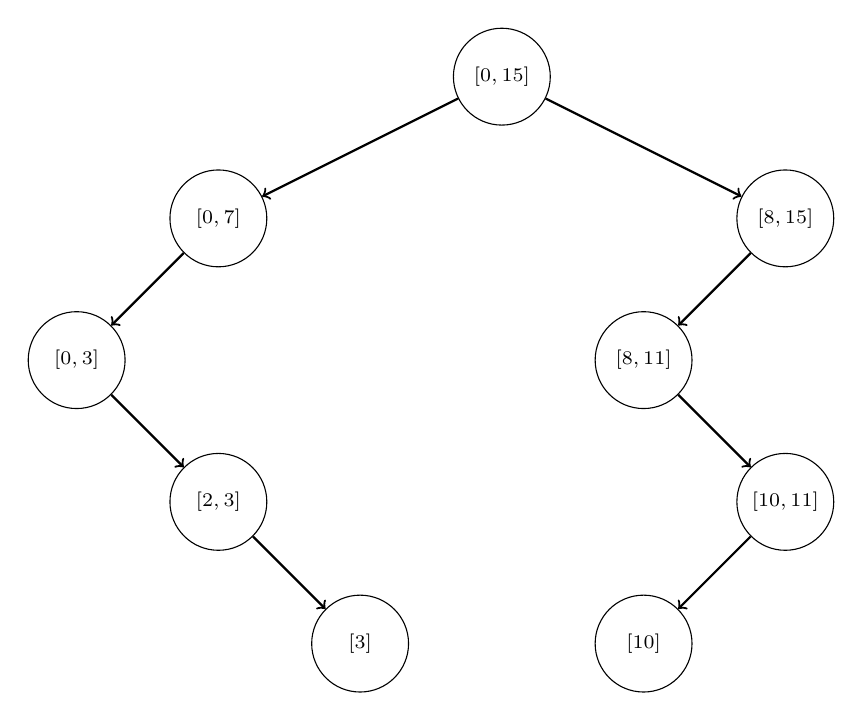
\begin{tikzpicture}[scale=0.9]
\scriptsize
\node[draw, circle,minimum size=35pt] (1) at (0,0) {$[0,15]$};
\node[draw, circle,minimum size=35pt] (2) at (-4,-2) {$[0,7]$};
\node[draw, circle,minimum size=35pt] (3) at (-6,-4) {$[0,3]$};
\node[draw, circle,minimum size=35pt] (4) at (-4,-6) {$[2,3]$};
\node[draw, circle,minimum size=35pt] (5) at (-2,-8) {$[3]$};
\node[draw, circle,minimum size=35pt] (6) at (4,-2) {$[8,15]$};
\node[draw, circle,minimum size=35pt] (7) at (2,-4) {$[8,11]$};
\node[draw, circle,minimum size=35pt] (8) at (4,-6) {$[10,11]$};
\node[draw, circle,minimum size=35pt] (9) at (2,-8) {$[10]$};

\path[draw,thick,->] (1) -- (2);
\path[draw,thick,->] (2) -- (3);
\path[draw,thick,->] (3) -- (4);
\path[draw,thick,->] (4) -- (5);

\path[draw,thick,->] (1) -- (6);
\path[draw,thick,->] (6) -- (7);
\path[draw,thick,->] (7) -- (8);
\path[draw,thick,->] (8) -- (9);
\end{tikzpicture}
\end{center}

Түбір төбеден жапырақ төбеге дейінгі жол 
$O(\log n)$ төбеден тұрады. Сондықтан да әр операция
дараққа көп дегенде $O(\log n)$ жаңа төбелер қосады.
Осылайша $k$ операциядан кейін, дарақ ең көбі 
$O(k \log n)$ төбелерден тұрады.

% Any path from the root node to a leaf contains
% $O(\log n)$ nodes,
% so each operation adds at most $O(\log n)$
% new nodes to the tree.
% Thus, after $k$ operations, the tree contains
% at most $O(k \log n)$ nodes.

Мына жайтты ескергеніміз жөн: жаңартылатын барлық
элементтерді алгоритмнің басында  білетін болсақ, бізге динамикалық кесінділер дарағы
керек болмас еді. Өйткені біз индекстерді сығымдау арқылы
қарапайым кесінділер дарағын (9.4-тарау)
қолданар едік. Алайда, егер индекстер алгоритмнің жұмысы барысында туындаса, бұл мүмкін болмайды. 

% Note that if we know all elements to be updated
% at the beginning of the algorithm,
% a dynamic segment tree is not necessary,
% because we can use an ordinary segment tree with
% index compression (Chapter 9.4).
% However, this is not possible when the indices
% are generated during the algorithm.

\subsubsection{Ұзақ сақталушы кесінділер дарағы}

\index{ұзақ сақталушы кесінділер дарағы}

Динамикалық іске асыру арқылы
\emph{жаңартулар тарихын} сақтайтын \key{ұзақ сақталушы кесінділер дарағын}
да құрыстыруымызға болады. Ол арқылы біз алгоритмнің 
барысында дарақта болған барлық нұсқаларға оңтайлы жүгіне
аламыз. 

% Using a dynamic implementation,
% it is also possible to create a
% \key{persistent segment tree} that stores
% the \emph{modification history} of the tree.
% In such an implementation, we can
% efficiently access
% all versions of the tree that have
% existed during the algorithm.

Модификациялау тарихы қолжетімді болса, дарақтың 
кез келген алдыңғы версияларына қарапайым кесінділер 
дарағы сияқты сұратымдар жасауымызға болады. Өйткені әр дарақтың толық құрылымы сақталып тұрады. Сондай-ақ біз бұрынғы дарақтардың  негізінде жаңа дарақтар құрып, 
оларды дербес өзгерте аламыз. 

% When the modification history is available,
% we can perform queries in any previous tree
% like in an ordinary segment tree, because the
% full structure of each tree is stored.
% We can also create new trees based on previous
% trees and modify them independently.

Қызыл төбелері өзгеретін, ал басқа төбелері өзгеріссіз қалатын келесі жаңартулар тізбегін қарастырайық:

% Consider the following sequence of updates,
% where red nodes change
% and other nodes remain the same:

\begin{center}
\begin{tikzpicture}[scale=0.8]
\node[draw, circle,minimum size=13pt] (1a) at (3,0) {};
\node[draw, circle,minimum size=13pt] (2a) at (2,-1) {};
\node[draw, circle,minimum size=13pt] (3a) at (4,-1) {};
\node[draw, circle,minimum size=13pt] (4a) at (1.5,-2) {};
\node[draw, circle,minimum size=13pt] (5a) at (2.5,-2) {};
\node[draw, circle,minimum size=13pt] (6a) at (3.5,-2) {};
\node[draw, circle,minimum size=13pt] (7a) at (4.5,-2) {};
\path[draw,thick,->] (1a) -- (2a);
\path[draw,thick,->] (1a) -- (3a);
\path[draw,thick,->] (2a) -- (4a);
\path[draw,thick,->] (2a) -- (5a);
\path[draw,thick,->] (3a) -- (6a);
\path[draw,thick,->] (3a) -- (7a);

\node[draw, circle,minimum size=13pt,fill=red] (1b) at (3+5,0) {};
\node[draw, circle,minimum size=13pt,fill=red] (2b) at (2+5,-1) {};
\node[draw, circle,minimum size=13pt] (3b) at (4+5,-1) {};
\node[draw, circle,minimum size=13pt] (4b) at (1.5+5,-2) {};
\node[draw, circle,minimum size=13pt,fill=red] (5b) at (2.5+5,-2) {};
\node[draw, circle,minimum size=13pt] (6b) at (3.5+5,-2) {};
\node[draw, circle,minimum size=13pt] (7b) at (4.5+5,-2) {};
\path[draw,thick,->] (1b) -- (2b);
\path[draw,thick,->] (1b) -- (3b);
\path[draw,thick,->] (2b) -- (4b);
\path[draw,thick,->] (2b) -- (5b);
\path[draw,thick,->] (3b) -- (6b);
\path[draw,thick,->] (3b) -- (7b);

\node[draw, circle,minimum size=13pt,fill=red] (1c) at (3+10,0) {};
\node[draw, circle,minimum size=13pt] (2c) at (2+10,-1) {};
\node[draw, circle,minimum size=13pt,fill=red] (3c) at (4+10,-1) {};
\node[draw, circle,minimum size=13pt] (4c) at (1.5+10,-2) {};
\node[draw, circle,minimum size=13pt] (5c) at (2.5+10,-2) {};
\node[draw, circle,minimum size=13pt] (6c) at (3.5+10,-2) {};
\node[draw, circle,minimum size=13pt,fill=red] (7c) at (4.5+10,-2) {};
\path[draw,thick,->] (1c) -- (2c);
\path[draw,thick,->] (1c) -- (3c);
\path[draw,thick,->] (2c) -- (4c);
\path[draw,thick,->] (2c) -- (5c);
\path[draw,thick,->] (3c) -- (6c);
\path[draw,thick,->] (3c) -- (7c);

\node at (3,-3) {1–қадам};
\node at (3+5,-3) {2-қадам};
\node at (3+10,-3) {3-қадам};
\end{tikzpicture}
\end{center}
Әр жаңартудан кейін төбелердің көбі өзгеріссіз қалады, сондықтан модификация тарихын сақтаудың ықшам тәсілі дарақтың әр тарихи версиясын жаңа төбелер мен алдыңғы дарақ ішдарақтарының комбинациялары түрінде ұсынудан тұрады. 
Бұл мысалда жаңартулар тарихы келесі ретпен сақталады:

% After each update, most nodes of the tree
% remain the same,
% so an efficient way to store the modification history
% is to represent each tree in the history as a combination
% of new nodes and subtrees of previous trees.
% In this example, the modification history can be
% stored as follows:
\begin{center}
\begin{tikzpicture}[scale=0.8]
\path[use as bounding box] (0, 1) rectangle (16, -3.5);

\node[draw, circle,minimum size=13pt] (1a) at (3,0) {};
\node[draw, circle,minimum size=13pt] (2a) at (2,-1) {};
\node[draw, circle,minimum size=13pt] (3a) at (4,-1) {};
\node[draw, circle,minimum size=13pt] (4a) at (1.5,-2) {};
\node[draw, circle,minimum size=13pt] (5a) at (2.5,-2) {};
\node[draw, circle,minimum size=13pt] (6a) at (3.5,-2) {};
\node[draw, circle,minimum size=13pt] (7a) at (4.5,-2) {};
\path[draw,thick,->] (1a) -- (2a);
\path[draw,thick,->] (1a) -- (3a);
\path[draw,thick,->] (2a) -- (4a);
\path[draw,thick,->] (2a) -- (5a);
\path[draw,thick,->] (3a) -- (6a);
\path[draw,thick,->] (3a) -- (7a);

\node[draw, circle,minimum size=13pt,fill=red] (1b) at (3+5,0) {};
\node[draw, circle,minimum size=13pt,fill=red] (2b) at (2+5,-1) {};
\node[draw, circle,minimum size=13pt,fill=red] (5b) at (2.5+5,-2) {};
\path[draw,thick,->] (1b) -- (2b);

\draw[thick,->] (1b) .. controls (3+5+2,0-1) and (3+5,2.5) .. (3a);

\draw[thick,->] (2b) .. controls (2+5-0.5,-1-0.5) and (2,4.5) .. (4a);


\path[draw,thick,->] (2b) -- (5b);

\node[draw, circle,minimum size=13pt,fill=red] (1c) at (3+10,0) {};
\node[draw, circle,minimum size=13pt,fill=red] (3c) at (4+10,-1) {};
\node[draw, circle,minimum size=13pt,fill=red] (7c) at (4.5+10,-2) {};
\path[draw,thick,->] (1c) -- (2b);
\path[draw,thick,->] (1c) -- (3c);

\draw[thick,->] (3c) .. controls (2.5+5,-3) and (3.5,-3) .. (6a);

\path[draw,thick,->] (3c) -- (7c);

\node at (3,-3) {1-қадам};
\node at (3+5,-3) {2-қадам};
\node at (3+10,-3) {3-қадам};
\end{tikzpicture}
\end{center}

Әр алдыңғы дарақтың құрылымын сәйкес түбірден бастап, нұсқағыштарға ілесе отырып, қалпына келтіруімізге болады. Әр операция  
дараққа жаңа $O(\log n)$ төбе қосатындықтан,
дарақтың барлық жаңарту тарихын сақтай аламыз. 

% The structure of each previous tree can be
% reconstructed by following the pointers
% starting at the corresponding root node.
% Since each operation
% adds only $O(\log n)$ new nodes to the tree,
% it is possible to store the full modification history of the tree.

\section{Деректер құрылымы}

Кесінділер дарағындағы төбелер 
жекелеген мәндердің орнына сәйкес аралық бойынша ақпараттан тұратын  
\emph{деректер құрылымын} да сақтай алады.
Ондай дарақта операциялар $O(f(n) \log n)$ уақыт алады,
мұндағы $f(n)$ -- операция барысында бір төбені өңдеуге кететін уақыты. 

% Instead of single values, nodes in a segment tree
% can also contain \emph{data structures} that maintain information
% about the corresponding ranges.
% In such a tree, the operations take
% $O(f(n) \log n)$ time, where $f(n)$ is
% the time needed for processing a single node during an operation.

Үлгі ретінде ''$[a,b]$ аралықта $x$ элементі қанша рет кездеседі?'' -
деген сұратымдарды қолдайтын кесінділер дарағын қарастырайық.
Мысалы, 1 элементі келесі аралықта 3 рет кездеседі:

% As an example, consider a segment tree that
% supports queries of the form
% ''how many times does an element $x$ appear
% in the range $[a,b]$?''
% For example, the element 1 appears three times
% in the following range:

\begin{center}
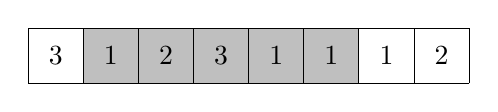
\begin{tikzpicture}[scale=0.7]
\fill[lightgray] (1,0) rectangle (6,1);
\draw (0,0) grid (8,1);

\node[anchor=center] at (0.5, 0.5) {3};
\node[anchor=center] at (1.5, 0.5) {1};
\node[anchor=center] at (2.5, 0.5) {2};
\node[anchor=center] at (3.5, 0.5) {3};
\node[anchor=center] at (4.5, 0.5) {1};
\node[anchor=center] at (5.5, 0.5) {1};
\node[anchor=center] at (6.5, 0.5) {1};
\node[anchor=center] at (7.5, 0.5) {2};
\end{tikzpicture}
\end{center}

Осындай сұратымдарды қолдау үшін 
әр төбеде кез келген $x$ саны сәйкес аралықта қанша рет 
кездесетінін айтып беретін деректер құрылымы бар
кесінділер дарағын құрастырамыз. Осы дарақты қолдана отырып, аралыққа кіретін төбелердің жауаптарын 
біріктіру арқылы сұратымның жауабын алуымызға болады. 

% To support such queries, we build a segment tree
% where each node is assigned a data structure
% that can be asked how many times any element $x$
% appears in the corresponding range.
% Using this tree,
% the answer to a query can be calculated
% by combining the results from the nodes
% that belong to the range.

Мысалы, келесі кесінділер дарағы үстідегі жиымға 
сәйкес келеді:
% For example, the following segment tree
% corresponds to the above array:
\begin{center}
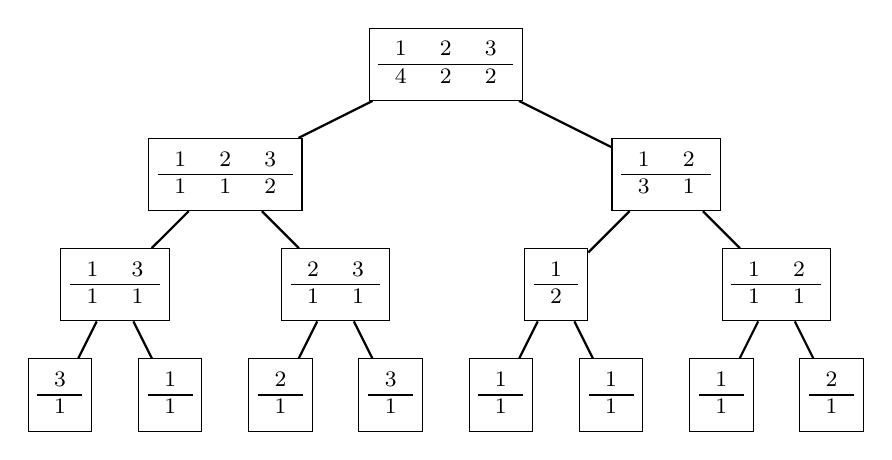
\begin{tikzpicture}[scale=0.7]

\node[draw, rectangle] (a) at (1,2.5)
{
\footnotesize
\begin{tabular}{r}
3 \\
\hline
1 \\
\end{tabular}};
\node[draw, rectangle] (b) at (3,2.5)
{
\footnotesize
\begin{tabular}{r}
1 \\
\hline
1 \\
\end{tabular}};
\node[draw, rectangle] (c) at (5,2.5)
{
\footnotesize
\begin{tabular}{r}
2 \\
\hline
1 \\
\end{tabular}};
\node[draw, rectangle] (d) at (7,2.5)
{
\footnotesize
\begin{tabular}{r}
3 \\
\hline
1 \\
\end{tabular}};
\node[draw, rectangle] (e) at (9,2.5)
{
\footnotesize
\begin{tabular}{r}
1 \\
\hline
1 \\
\end{tabular}};
\node[draw, rectangle] (f) at (11,2.5)
{
\footnotesize
\begin{tabular}{r}
1 \\
\hline
1 \\
\end{tabular}};
\node[draw, rectangle] (g) at (13,2.5)
{
\footnotesize
\begin{tabular}{r}
1 \\
\hline
1 \\
\end{tabular}};
\node[draw, rectangle] (h) at (15,2.5)
{
\footnotesize
\begin{tabular}{r}
2 \\
\hline
1 \\
\end{tabular}};

\node[draw, rectangle] (i) at (2,4.5)
{
\footnotesize
\begin{tabular}{rr}
1 & 3 \\
\hline
1 & 1 \\
\end{tabular}};
\path[draw,thick,-] (i) -- (a);
\path[draw,thick,-] (i) -- (b);
\node[draw, rectangle] (j) at (6,4.5)
{
\footnotesize
\begin{tabular}{rr}
2 & 3 \\
\hline
1 & 1 \\
\end{tabular}};
\path[draw,thick,-] (j) -- (c);
\path[draw,thick,-] (j) -- (d);
\node[draw, rectangle] (k) at (10,4.5)
{
\footnotesize
\begin{tabular}{r}
1 \\
\hline
2 \\
\end{tabular}};
\path[draw,thick,-] (k) -- (e);
\path[draw,thick,-] (k) -- (f);
\node[draw, rectangle] (l) at (14,4.5)
{
\footnotesize
\begin{tabular}{rr}
1 & 2 \\
\hline
1 & 1 \\
\end{tabular}};
\path[draw,thick,-] (l) -- (g);
\path[draw,thick,-] (l) -- (h);

\node[draw, rectangle] (m) at (4,6.5)
{
\footnotesize
\begin{tabular}{rrr}
1 & 2 & 3 \\
\hline
1 & 1 & 2 \\
\end{tabular}};
\path[draw,thick,-] (m) -- (i);
\path[draw,thick,-] (m) -- (j);
\node[draw, rectangle] (n) at (12,6.5)
{
\footnotesize
\begin{tabular}{rr}
1 & 2 \\
\hline
3 & 1 \\
\end{tabular}};
\path[draw,thick,-] (n) -- (k);
\path[draw,thick,-] (n) -- (l);

\node[draw, rectangle] (o) at (8,8.5)
{
\footnotesize
\begin{tabular}{rrr}
1 & 2 & 3 \\
\hline
4 & 2 & 2 \\
\end{tabular}};
\path[draw,thick,-] (o) -- (m);
\path[draw,thick,-] (o) -- (n);
\end{tikzpicture}
\end{center}

Дарақты әр төбеде \texttt{map} құрылымы болатындай етіп құрастыра аламыз. Ондай жағдайда
әр төбені өңдеуге $O(\log n)$ уақыт жұмсалады, демек
сұратымның жалпы уақытша күрделігі $O(\log^2 n)$ болады.
Дарақ $O(n \log n)$ жадыны қолданады, өйткені дарақта $O(\log n)$ деңгей, ал 
әр деңгейде $O(n)$ элемент бар. 

% We can build the tree so
% that each node contains a \texttt{map} structure.
% In this case, the time needed for processing each
% node is $O(\log n)$, so the total time complexity
% of a query is $O(\log^2 n)$.
% The tree uses $O(n \log n)$ memory,
% because there are $O(\log n)$ levels
% and each level contains
% $O(n)$ elements.

\section{Екі өлшемділік}

\index{екі өлшемді кесінділер дарағы}

\key{Екі өлшемді кесінділер дарағы} екі 
өлшемді жиымның тіктөртбұрышты 
ішжиымдарына қатысты сұратымдарды қолдайды. 
Ондай дарақты кірістірілген кесінділер дарағы арқылы 
жүзеге асыра аламыз. Үлкен дарақ жиымның жолдарына
сәйкес келеді және әр төбе бағанға сәйкес кішкентай дарақты қамтиды. 

% A \key{two-dimensional segment tree} supports
% queries related to rectangular subarrays
% of a two-dimensional array.
% Such a tree can be implemented as
% nested segment trees: a big tree corresponds to the
% rows of the array, and each node contains a small tree
% that corresponds to a column.

Мысалы: 
\begin{center}
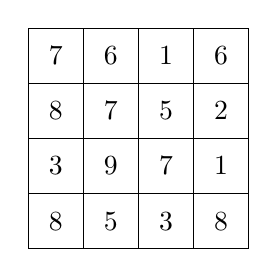
\begin{tikzpicture}[scale=0.7]
\draw (0,0) grid (4,4);

\node[anchor=center] at (0.5, 0.5) {8};
\node[anchor=center] at (1.5, 0.5) {5};
\node[anchor=center] at (2.5, 0.5) {3};
\node[anchor=center] at (3.5, 0.5) {8};

\node[anchor=center] at (0.5, 1.5) {3};
\node[anchor=center] at (1.5, 1.5) {9};
\node[anchor=center] at (2.5, 1.5) {7};
\node[anchor=center] at (3.5, 1.5) {1};

\node[anchor=center] at (0.5, 2.5) {8};
\node[anchor=center] at (1.5, 2.5) {7};
\node[anchor=center] at (2.5, 2.5) {5};
\node[anchor=center] at (3.5, 2.5) {2};

\node[anchor=center] at (0.5, 3.5) {7};
\node[anchor=center] at (1.5, 3.5) {6};
\node[anchor=center] at (2.5, 3.5) {1};
\node[anchor=center] at (3.5, 3.5) {6};
\end{tikzpicture}
\end{center}
жиымның кез келген ішжиымын
төмендегі кесінділер дарағы арқылы есептеуімізге болады:
% the sum of any subarray
% can be calculated
% from the following segment tree:
\begin{center}
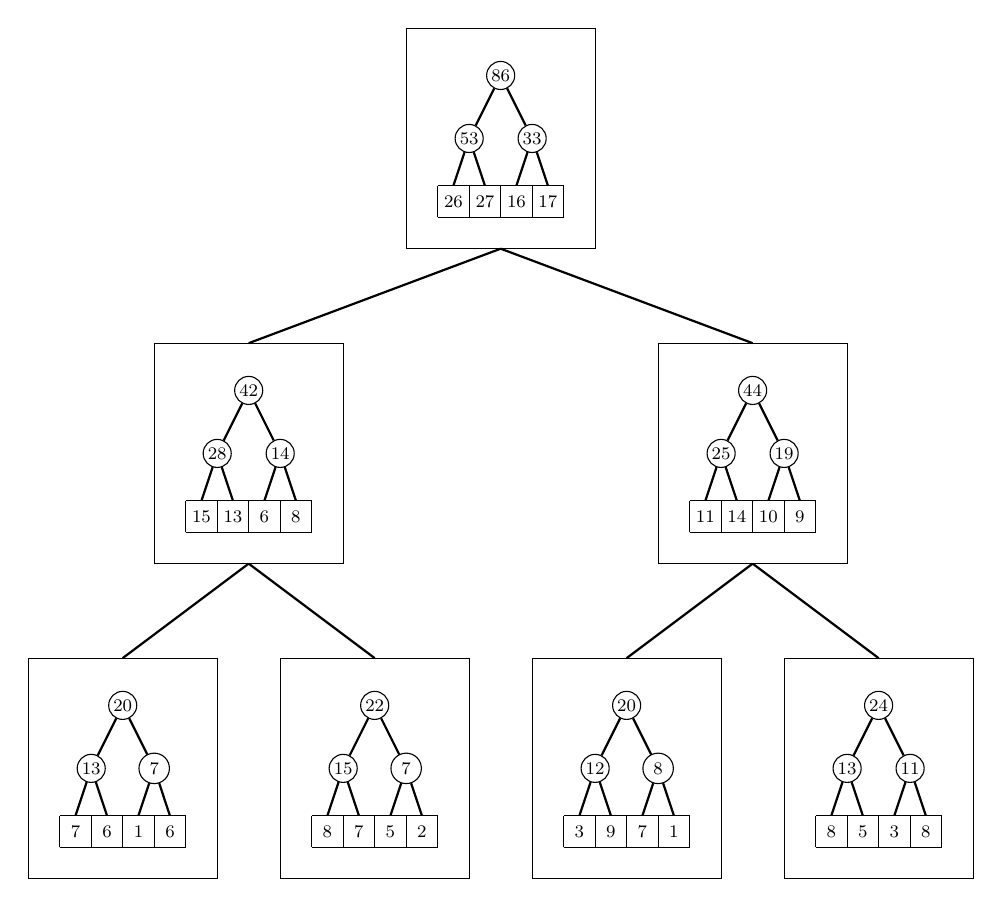
\begin{tikzpicture}[scale=0.4]
\footnotesize
\begin{scope}[shift={(-12,0)}]
\draw (-1,-1) rectangle (5,6);
\draw (0,0) grid (4,1);
\node[anchor=center,scale=0.8] at (0.5, 0.5) {7};
\node[anchor=center,scale=0.8] at (1.5, 0.5) {6};
\node[anchor=center,scale=0.8] at (2.5, 0.5) {1};
\node[anchor=center,scale=0.8] at (3.5, 0.5) {6};

\node[draw, circle,scale=0.8,inner sep=1pt] (a) at (1,2.5) {13};
\path[draw,thick,-] (a) -- (0.5,1);
\path[draw,thick,-] (a) -- (1.5,1);
\node[draw, circle,scale=0.8,inner sep=2.5pt] (b) at (3,2.5) {7};
\path[draw,thick,-] (b) -- (2.5,1);
\path[draw,thick,-] (b) -- (3.5,1);

\node[draw, circle,scale=0.8,inner sep=1pt] (i) at (2,4.5) {20};
\path[draw,thick,-] (i) -- (a);
\path[draw,thick,-] (i) -- (b);
\end{scope}
\begin{scope}[shift={(-4,0)}]
\draw (-1,-1) rectangle (5,6);
\draw (0,0) grid (4,1);
\node[anchor=center,scale=0.8] at (0.5, 0.5) {8};
\node[anchor=center,scale=0.8] at (1.5, 0.5) {7};
\node[anchor=center,scale=0.8] at (2.5, 0.5) {5};
\node[anchor=center,scale=0.8] at (3.5, 0.5) {2};

\node[draw, circle,scale=0.8,inner sep=1pt] (a) at (1,2.5) {15};
\path[draw,thick,-] (a) -- (0.5,1);
\path[draw,thick,-] (a) -- (1.5,1);
\node[draw, circle,scale=0.8,inner sep=2.5pt] (b) at (3,2.5) {7};
\path[draw,thick,-] (b) -- (2.5,1);
\path[draw,thick,-] (b) -- (3.5,1);

\node[draw, circle,scale=0.8,inner sep=1pt] (i) at (2,4.5) {22};
\path[draw,thick,-] (i) -- (a);
\path[draw,thick,-] (i) -- (b);
\end{scope}
\begin{scope}[shift={(4,0)}]
\draw (-1,-1) rectangle (5,6);
\draw (0,0) grid (4,1);
\node[anchor=center,scale=0.8] at (0.5, 0.5) {3};
\node[anchor=center,scale=0.8] at (1.5, 0.5) {9};
\node[anchor=center,scale=0.8] at (2.5, 0.5) {7};
\node[anchor=center,scale=0.8] at (3.5, 0.5) {1};

\node[draw, circle,scale=0.8,inner sep=1pt] (a) at (1,2.5) {12};
\path[draw,thick,-] (a) -- (0.5,1);
\path[draw,thick,-] (a) -- (1.5,1);
\node[draw, circle,scale=0.8,inner sep=2.5pt] (b) at (3,2.5) {8};
\path[draw,thick,-] (b) -- (2.5,1);
\path[draw,thick,-] (b) -- (3.5,1);

\node[draw, circle,scale=0.8,inner sep=1pt] (i) at (2,4.5) {20};
\path[draw,thick,-] (i) -- (a);
\path[draw,thick,-] (i) -- (b);
\end{scope}
\begin{scope}[shift={(12,0)}]
\draw (-1,-1) rectangle (5,6);
\draw (0,0) grid (4,1);
\node[anchor=center,scale=0.8] at (0.5, 0.5) {8};
\node[anchor=center,scale=0.8] at (1.5, 0.5) {5};
\node[anchor=center,scale=0.8] at (2.5, 0.5) {3};
\node[anchor=center,scale=0.8] at (3.5, 0.5) {8};

\node[draw, circle,scale=0.8,inner sep=1pt] (a) at (1,2.5) {13};
\path[draw,thick,-] (a) -- (0.5,1);
\path[draw,thick,-] (a) -- (1.5,1);
\node[draw, circle,scale=0.8,inner sep=1pt] (b) at (3,2.5) {11};
\path[draw,thick,-] (b) -- (2.5,1);
\path[draw,thick,-] (b) -- (3.5,1);

\node[draw, circle,scale=0.8,inner sep=1pt] (i) at (2,4.5) {24};
\path[draw,thick,-] (i) -- (a);
\path[draw,thick,-] (i) -- (b);
\end{scope}
\begin{scope}[shift={(-8,10)}]
\draw (-1,-1) rectangle (5,6);
\draw (0,0) grid (4,1);
\node[anchor=center,scale=0.8] at (0.5, 0.5) {15};
\node[anchor=center,scale=0.8] at (1.5, 0.5) {13};
\node[anchor=center,scale=0.8] at (2.5, 0.5) {6};
\node[anchor=center,scale=0.8] at (3.5, 0.5) {8};

\node[draw, circle,scale=0.8,inner sep=1pt] (a) at (1,2.5) {28};
\path[draw,thick,-] (a) -- (0.5,1);
\path[draw,thick,-] (a) -- (1.5,1);
\node[draw, circle,scale=0.8,inner sep=1pt] (b) at (3,2.5) {14};
\path[draw,thick,-] (b) -- (2.5,1);
\path[draw,thick,-] (b) -- (3.5,1);

\node[draw, circle,scale=0.8,inner sep=1pt] (i) at (2,4.5) {42};
\path[draw,thick,-] (i) -- (a);
\path[draw,thick,-] (i) -- (b);
\end{scope}
\begin{scope}[shift={(8,10)}]
\draw (-1,-1) rectangle (5,6);
\draw (0,0) grid (4,1);
\node[anchor=center,scale=0.8] at (0.5, 0.5) {11};
\node[anchor=center,scale=0.8] at (1.5, 0.5) {14};
\node[anchor=center,scale=0.8] at (2.5, 0.5) {10};
\node[anchor=center,scale=0.8] at (3.5, 0.5) {9};

\node[draw, circle,scale=0.8,inner sep=1pt] (a) at (1,2.5) {25};
\path[draw,thick,-] (a) -- (0.5,1);
\path[draw,thick,-] (a) -- (1.5,1);
\node[draw, circle,scale=0.8,inner sep=1pt] (b) at (3,2.5) {19};
\path[draw,thick,-] (b) -- (2.5,1);
\path[draw,thick,-] (b) -- (3.5,1);

\node[draw, circle,scale=0.8,inner sep=1pt] (i) at (2,4.5) {44};
\path[draw,thick,-] (i) -- (a);
\path[draw,thick,-] (i) -- (b);
\end{scope}
\begin{scope}[shift={(0,20)}]
\draw (-1,-1) rectangle (5,6);
\draw (0,0) grid (4,1);
\node[anchor=center,scale=0.8] at (0.5, 0.5) {26};
\node[anchor=center,scale=0.8] at (1.5, 0.5) {27};
\node[anchor=center,scale=0.8] at (2.5, 0.5) {16};
\node[anchor=center,scale=0.8] at (3.5, 0.5) {17};

\node[draw, circle,scale=0.8,inner sep=1pt] (a) at (1,2.5) {53};
\path[draw,thick,-] (a) -- (0.5,1);
\path[draw,thick,-] (a) -- (1.5,1);
\node[draw, circle,scale=0.8,inner sep=1pt] (b) at (3,2.5) {33};
\path[draw,thick,-] (b) -- (2.5,1);
\path[draw,thick,-] (b) -- (3.5,1);

\node[draw, circle,scale=0.8,inner sep=1pt] (i) at (2,4.5) {86};
\path[draw,thick,-] (i) -- (a);
\path[draw,thick,-] (i) -- (b);
\end{scope}
\path[draw,thick,-] (2,19) -- (-6,16);
\path[draw,thick,-] (2,19) -- (10,16);
\path[draw,thick,-] (-6,9) -- (-10,6);
\path[draw,thick,-] (-6,9) -- (-2,6);
\path[draw,thick,-] (10,9) -- (6,6);
\path[draw,thick,-] (10,9) -- (14,6);
\end{tikzpicture}
\end{center}

Екі өлшемді кесінділер дарағының операциялары $O(\log^2 n)$ уақыт
алады. Себебі үлкен дарақ және әр кішкентай дарақ $O(\log n)$
деңгейлерден тұрады. Әр кіші дарақ $O(n)$ мәндерден тұратындықтан, дараққа $O(n^2)$ жады керек болады.

% The operations of a two-dimensional segment tree
% take $O(\log^2 n)$ time, because the big tree
% and each small tree consist of $O(\log n)$ levels.
% The tree requires $O(n^2)$ memory, because each
% small tree contains $O(n)$ values.
